% Digital Logic Report Template
% Created: 2019-09-13, John Miller

%==========================================================
%=========== Document Setup  ==============================

% Formatting defined by class file
\documentclass[11pt]{article}

% ---- Document formatting ----
\usepackage[margin=1in]{geometry}	% Narrower margins
\usepackage{booktabs}				% Nice formatting of tables
\usepackage{graphicx}				% Ability to include graphics

%\setlength\parindent{0pt}	% Do not indent first line of paragraphs 
\usepackage[parfill]{parskip}		% Line space b/w paragraphs
%	parfill option prevents last line of pgrph from being fully justified

% Parskip package adds too much space around titles, fix with this
\RequirePackage{titlesec}
\titlespacing\section{0pt}{8pt plus 4pt minus 2pt}{3pt plus 2pt minus 2pt}
\titlespacing\subsection{0pt}{4pt plus 4pt minus 2pt}{-2pt plus 2pt minus 2pt}
\titlespacing\subsubsection{0pt}{2pt plus 4pt minus 2pt}{-6pt plus 2pt minus 2pt}

% ---- Hyperlinks ----
\usepackage[colorlinks=true,urlcolor=blue]{hyperref}	% For URL's. Automatically links internal references.

% ---- Code listings ----
\usepackage{listings} 					% Nice code layout and inclusion
\usepackage[usenames,dvipsnames]{xcolor}	% Colors (needs to be defined before using colors)

% Define custom colors for listings
\definecolor{listinggray}{gray}{0.98}		% Listings background color
\definecolor{rulegray}{gray}{0.7}			% Listings rule/frame color

% Style for Verilog
\lstdefinestyle{Verilog}{
	language=Verilog,					% Verilog
	backgroundcolor=\color{listinggray},	% light gray background
	rulecolor=\color{blue}, 			% blue frame lines
	frame=tb,							% lines above & below
	linewidth=\columnwidth, 			% set line width
	basicstyle=\small\ttfamily,	% basic font style that is used for the code	
	breaklines=true, 					% allow breaking across columns/pages
	tabsize=3,							% set tab size
	commentstyle=\color{gray},	% comments in italic 
	stringstyle=\upshape,				% strings are printed in normal font
	showspaces=false,					% don't underscore spaces
}

% How to use: \Verilog[listing_options]{file}
\newcommand{\Verilog}[2][]{%
	\lstinputlisting[style=Verilog,#1]{#2}
}




%======================================================
%=========== Body  ====================================
\begin{document}

\title{ELC 2137 Lab 09: ALU with Input Register }
\author{Sebastian Lopez}
\maketitle

\section*{Summary}

In this lab I explain the difference between combinational and regular sequential logic. I also describe the operation of an SR latch, D latch, D flip-flop, and D register, as well as the differences in Verilog procedural blocks for combinational versus sequential logic. Lastly, I imported and modified modules from a previous project, and use them to design a modular system.

\section*{Expected results tables}

\begin{table*}[ht]\centering
	\caption{\textit{register} expected results table}
	\label{ALU:tbl:register_ERT}\medskip
	\begin{tabular}{l|rrrrrrrrrrr}
		Time (ns): & 0-5 & 5-10 & 10-15 & 15-20 & 20-25 & 25-30 & 30-35 & 35-40 & 40-45 & 45-50 & 50-55 \\
		\midrule
		D (hex) & 0 & 0 	  & A & A & 3 	    & 3 	  & 0 	    & 0 & 0$\to$6 & 6 & 6 \\
		clk     & 0 & 1 	  & 0 & 1 & 0 	    & 1 	  & 0 	    & 1 & 0 	  & 1 & 0 \\
		en  	& 0 & 0 	  & 1 & 1 & 1$\to$0 & 0$\to$1 & 1$\to$0 & 0 & 0$\to$1 & 1 & 1 \\
		rst 	& 0 & 0$\to$1 & 0 & 0 & 0 		& 0 	  & 0		& 0 & 0		  & 0 & 0 \\
		\midrule
		Q (hex) & X & X$\to$0 & 0$\to$A & A & A & A & A & A & A & A$\to$6 & 6 \\
		\bottomrule
	\end{tabular}
\end{table*}

\begin{table*}[ht]\centering
	\caption{\textit{alu} expected results table skeleton}
	\label{ALU:tbl:alu_ERT}\medskip
	\begin{tabular}{l|rrrrrr}
		Time (ns): & 0-10 & 10-20 & 20-30 & 30-40 & 40-50 & 50-60 \\
		\midrule
		in0 & 1  & 3 & 5 & 7 & 9 & b \\
		in1 & 2  & 4 & 6 & 8 & a & c \\
		op & 0  & 1 & 2 & 3 & 4 & 5 \\
		\midrule
		out & 3  & ff & 4 & 0f & 3 & b \\
		\bottomrule
	\end{tabular}
\end{table*}

\section*{Code}

\begin{lstlisting}[style=Verilog,
caption=Register Code,
label=code:ex 
]
`timescale 1ns / 1ps
// Sebastian Lopez  ELC 2137, 2020-04-02

module register #(parameter N = 1)
(
input clk, rst, en, 
input [N - 1:0] D, 
output reg [N - 1:0] Q
); 

always @(posedge clk, posedge rst)
begin 
if (rst==1)
Q <= 0; 
else if (en==1)
Q <= D;

end 
endmodule // register 
\end{lstlisting}

\begin{lstlisting}[style=Verilog,
caption=ALU Code,
label=code:ex 
]
`timescale 1ns / 1ps
// Sebastian Lopez  ELC 2137, 2020-04-02

module ALU #( parameter N = 8)(

input [N - 1:0] in0 ,
input [N - 1:0] in1 ,
input [3:0] op,
output reg [N -1:0] out
) ;

parameter ADD = 0;
parameter SUB = 1;
parameter AND = 2;
parameter OR = 3;
parameter XOR  =4;

always @ *
begin
case (op)
ADD : out = in0 + in1 ;
SUB: out = in0 - in1; 
AND: out = in0 & in1; 
OR: out = in0 | in1;
XOR: out = in0 ^ in1; 

default : out = in0 ;
endcase

end
endmodule // ALU
\end{lstlisting}

\begin{lstlisting}[style=Verilog,
caption=Top Lab9 Code,
label=code:ex 
]
`timescale 1ns / 1ps
// Sebastian Lopez  ELC 2137, 2020-04-02

module top_lab9 #( parameter N = 8)(

input btnU, btnD, clk, btnC,
input [11:0] sw,
output [15:0] led 
);

wire [7:0] reg1_out, ALU1_out, reg2_out;

register #(.N(8)) r1( 
.D(sw [7:0]), .en(btnD), .clk(clk), .rst(btnC),
.Q(reg1_out));

assign led [7:0] = reg1_out; 

ALU #(.N(8))  a1(
.in1(reg1_out), .in0(sw[7:0]), .op(sw[11:8]), 
.out(ALU1_out));

register #(.N(8))  r2(
.D(ALU1_out), .en(btnU), .clk(clk), .rst(btnC), 
.Q(reg2_out));

assign led [15:8] = reg2_out; 


endmodule // Top Lab9
\end{lstlisting}

\begin{lstlisting}[style=Verilog,
caption=Register test Code,
label=code:ex 
]
`timescale 1ns / 1ps
// Sebastian Lopez  ELC 2137, 2020-04-02

module register_test();

reg [3:0] D ;
reg clk , en , rst ;
wire [3:0] Q ;

register #(.N(4)) r(.D(D) ,.clk(clk),
.en(en), .rst(rst), .Q(Q)) ;

always begin
clk = ~ clk ; #5;
end

initial begin
clk = 0; en = 0; rst = 0; D = 4'h0 ; #7;
rst = 1; #3;

D = 4'hA ; en = 1; rst = 0; #10;
D = 4'h3 ;   #2;
en = 0;      #5;
en = 1;      #3;
D = 4'h0 ;   #2;
en = 0;      #10;
en = 1;      #2;
D = 4'h6 ;   #11;
$finish ;

end
endmodule // register_test
\end{lstlisting}

\begin{lstlisting}[style=Verilog,
caption=ALU Test Code,
label=code:ex 
]
`timescale 1ns / 1ps
// Sebastian Lopez  ELC 2137, 2020-04-02

module ALU_test();

reg [7:0] in0;
reg [7:0] in1;
reg [3:0] op;
wire [7:0] out;

ALU #(.N(8)) a(.in0(in0) ,.in1(in1),.op(op),
.out(out)) ;
initial begin 

op = 0; 
in0 = 1; 
in1 = 2;
#10 
op = 1; 
in0 = 3; 
in1 = 4;
#10 
op = 2; 
in0 = 5; 
in1 = 6;
#10 
op = 3; 
in0 = 7; 
in1 = 8;
#10 
op = 4; 
in0 = 9; 
in1 = 10;
#10 
op = 5; 
in0 = 11; 
in1 = 12;
#10
$finish; 

end
endmodule // ALU_test
\end{lstlisting}

\section*{Results}

\begin{figure}[ht]\centering	
	
	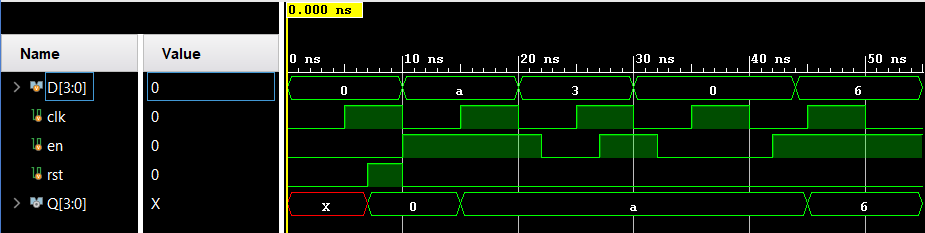
\includegraphics[width=1\textwidth,angle=0,origin=c]{register_test.PNG}
	\caption{Register Waveform}
	\label{fig:sim_with_table}
	
\end{figure}

\begin{figure}[ht]\centering
	
	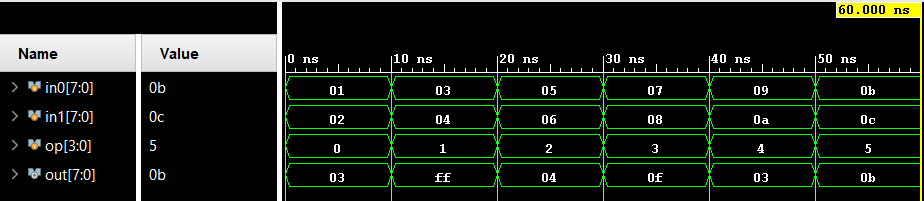
\includegraphics[width=1\textwidth,angle=0,origin=c]{ALU_test.PNG}
	\caption{ALU Waveform}
	\label{fig:sim_with_table}
	
\end{figure}

\begin{figure}[ht]\centering	
	
	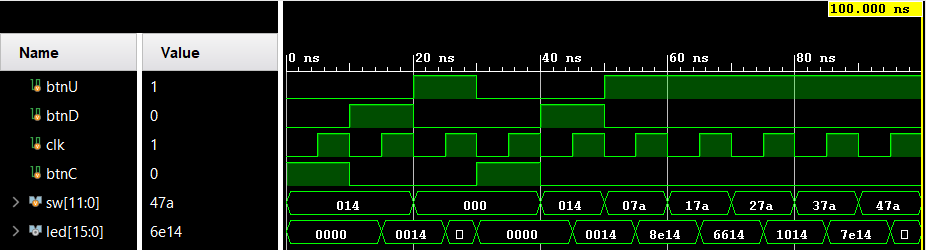
\includegraphics[width=1\textwidth,angle=0,origin=c]{basys3_lab9_behavior.PNG}
	\caption{Basys 3 Lab 9 Behavior Waveform}
	\label{fig:sim_with_table}
	
\end{figure}

\end{document}
